\chapter{Procedure}
\section{Equipment}
The necessary equipment for this lab is as follows:
\begin{itemize}
  \item 2 meter aluminum rod
  \item Table clamp
  \item Swivel clamp or $90^\circ$ Offset Clamp
  \item Meter Stick
  \item $\frac{1}{2}"$ and $\frac{3}{8}"$ steel ball
  \item Freefall Adapter - PASCO \#ME
  \item PASCO 750 Interface box
  \item PASCO Interface box power cord and SCSI Interface Card
  \item Laptop Computer w/ Data Studio
\end{itemize}

\section{Procedure}

\section{A. Apparatus Setup}

  Setup the apparatus as shown in the picture below. Make sure that the clamps are tight,
but not over tight. The clamp holding the apparatus should be tight enough to not allow
the apparatus to move around. Makre sure that the small thumb screw on the ball
clamp is on top.

\newpage 

\begin{figure}[htbp]
  \centerline{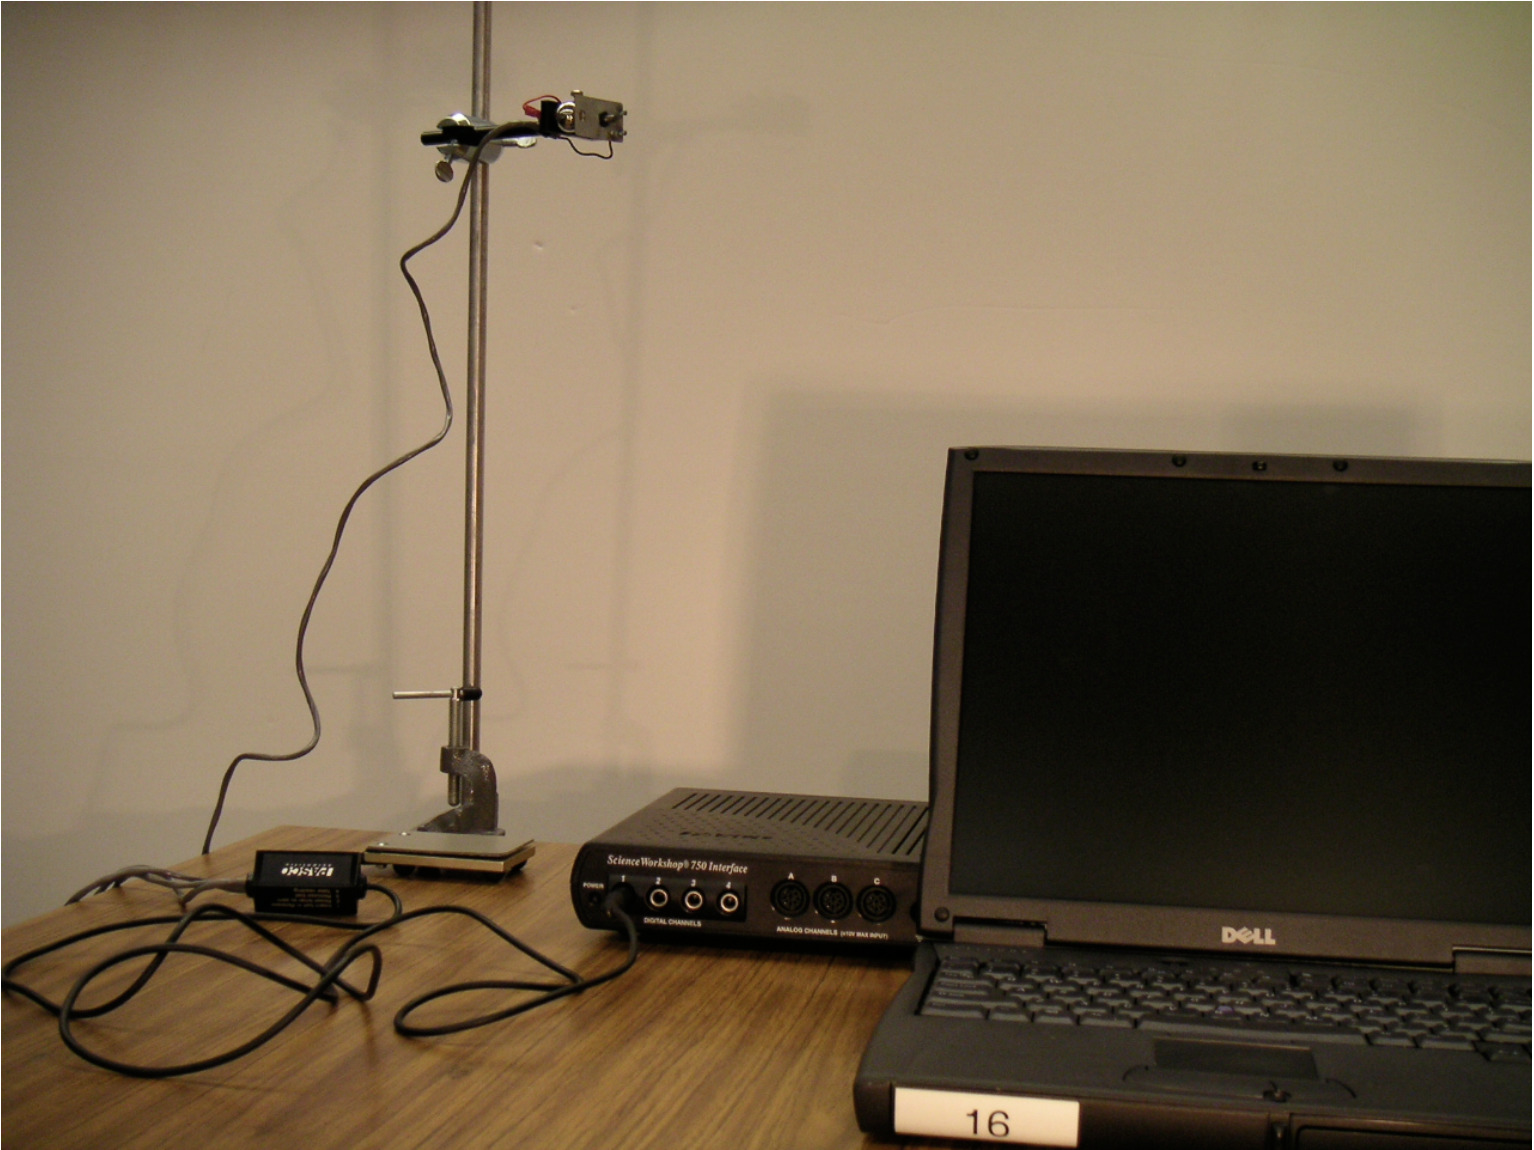
\includegraphics[scale=0.3]{resources/photo1.jpg}}
\end{figure}

  The apparatus consists of a small clamp that holds the metal ball and a steel rod;
it is designed to complete a circuit when the ball is installed. There is a plunger
that goes through the thin steel plate that has a retaining ring on both ends.
This plunger places pressure on the steel plate and holds the ball in place.

  Place the ball in the clamp, positioning it between the hole and the brass screw, pull on
plunger so that the retaining ring is exerting pressure on the steel plate. When there is enough
pressure on the plate to retain the ball, tighten the thumbscrew. The ball and apparatus are now
ready to be used.

  Position the floor plate directly beneath the ball clamp. Do a few test drops to make sure
that the ball solidly strikes the plate.

\textbf{Possible Pitfalls:} \\
  Due to the age of the apparatus, the circuit may be easily broken. It is possible, however, to
maneuver the ball so that the circuit remains closed.
  The thumbscrew must be tightly set; otherwise it will not hold the plunger. This means that
the slightest turn on the thumbscrew will release the plunger.

\section{B. Computer Setup}
  Provide power to the PASCO 750 Interface box, connect the box to the computer with the
SCSI cord and turn on the box, making sure the word “Honda” on the cord is facing upward when
it gets plugged into the computer. Only after you have turned on the PASCO 750 Interface
box 750 and plugged it into the computer, can you turn on the computer. (If you do not
perform these tasks in the above listed order, your computer will not recognize the PASCO
750 Interface box.) When the computer is first turned on, it may have a Found New Hardware
window open. If so, just ignore the window and proceed with the steps below.
  Double-Click on the \emph{Data Studio} icon on the desktop. The following screen should appear:

\begin{figure}[ht]
  \centerline{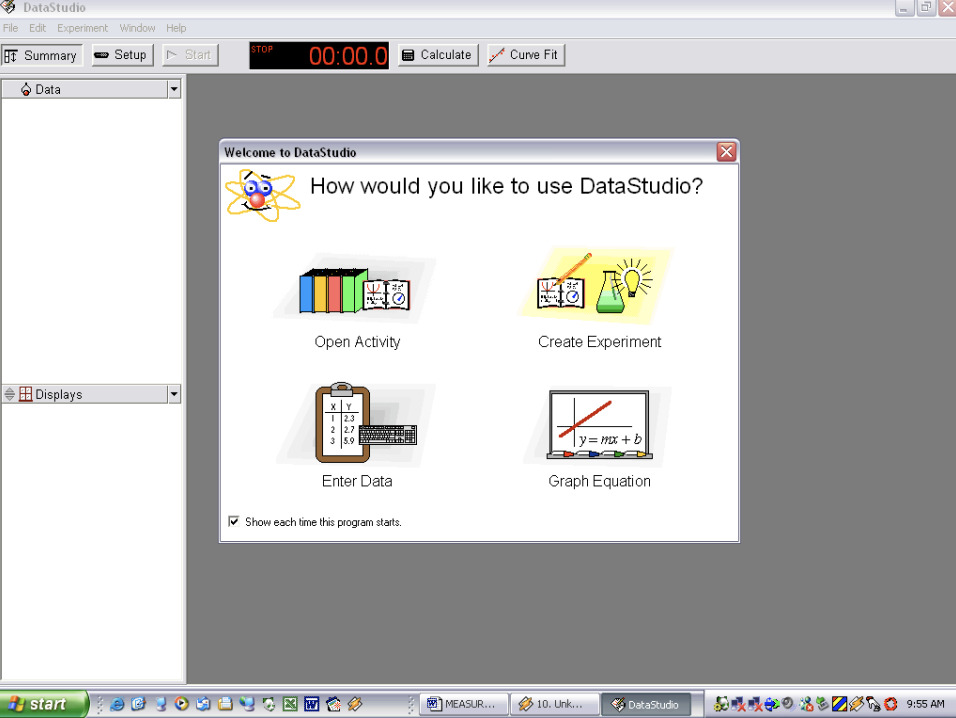
\includegraphics[scale=0.4]{resources/photo2.jpg}}
\end{figure}

Click \emph{Create Experiment}, if it cannot find the Interface box right away, click \emph{Scan}.
If it doesn’t find it after you have clicked \emph{Scan}, make sure that it is connected properly.
If it is connected properly and everything seems 
to be in order, restart the computer and the Interface box should load proper.
Once the Interface box is found, the following screen will appear:

\begin{figure}[ht]
  \centerline{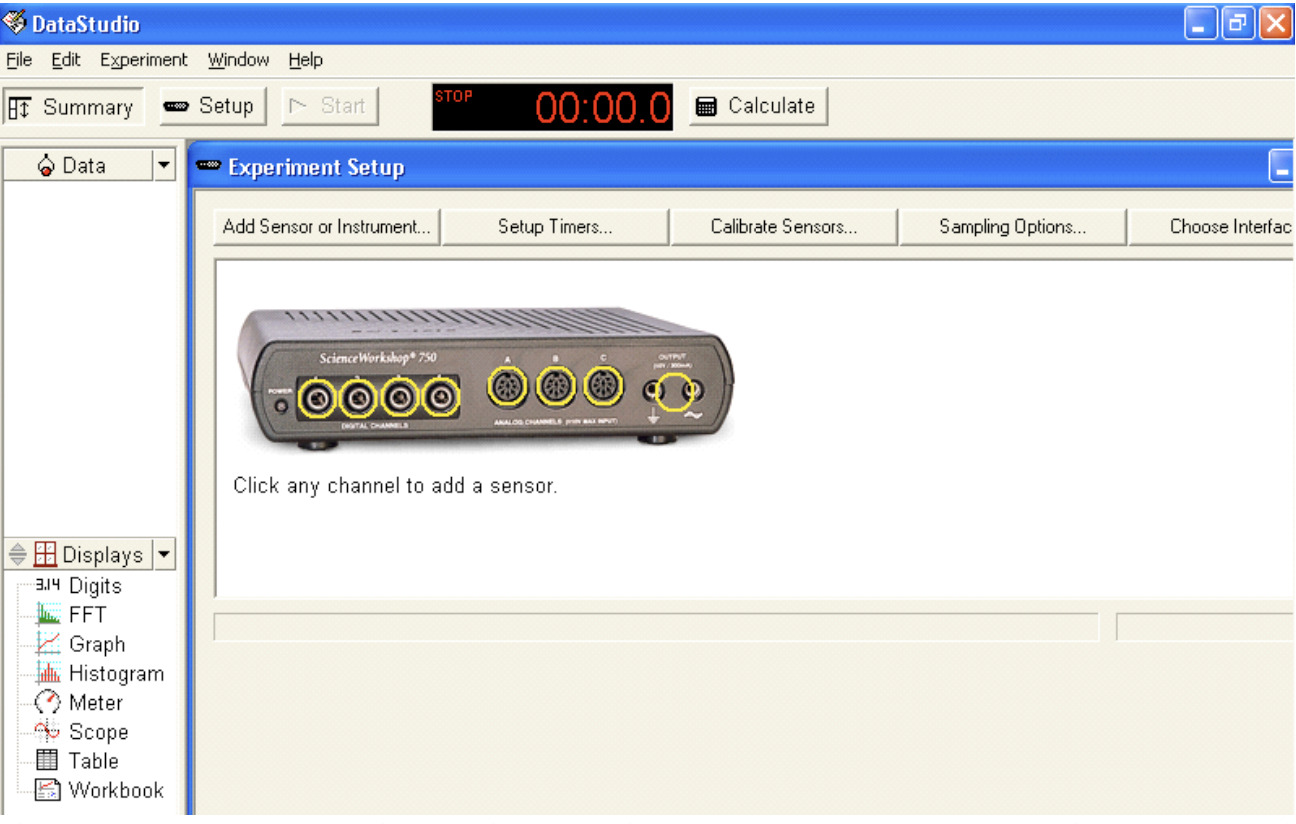
\includegraphics[scale=0.4]{resources/photo3.jpg}}
\end{figure}

This is your main window. This window contains a picture of the interface box you currently have attached, 
access to a list of sensors that can be attached to the Interface box, a toolbar to \emph{adjust} sensor options and other items.

Under \emph{Experiment Set-Up}, click \emph{Add Sensor or Instrument} and a window will open. 
Then click on the small black arrow near the top of the window to open a drop-down 
menu and select \emph{Scientific Workshop Digital Sensors}. Finally select \emph{Free-Fall Adapter} and click \emph{Ok}. See picture below.

In the \emph{Experiment Set-Up} window, on the bottom left corner of the window, 
click the \emph{Measurements} tab and de-select \emph{Acceleration, Ch 1 box}. As seen below.

\begin{figure}[hp]
  \centerline{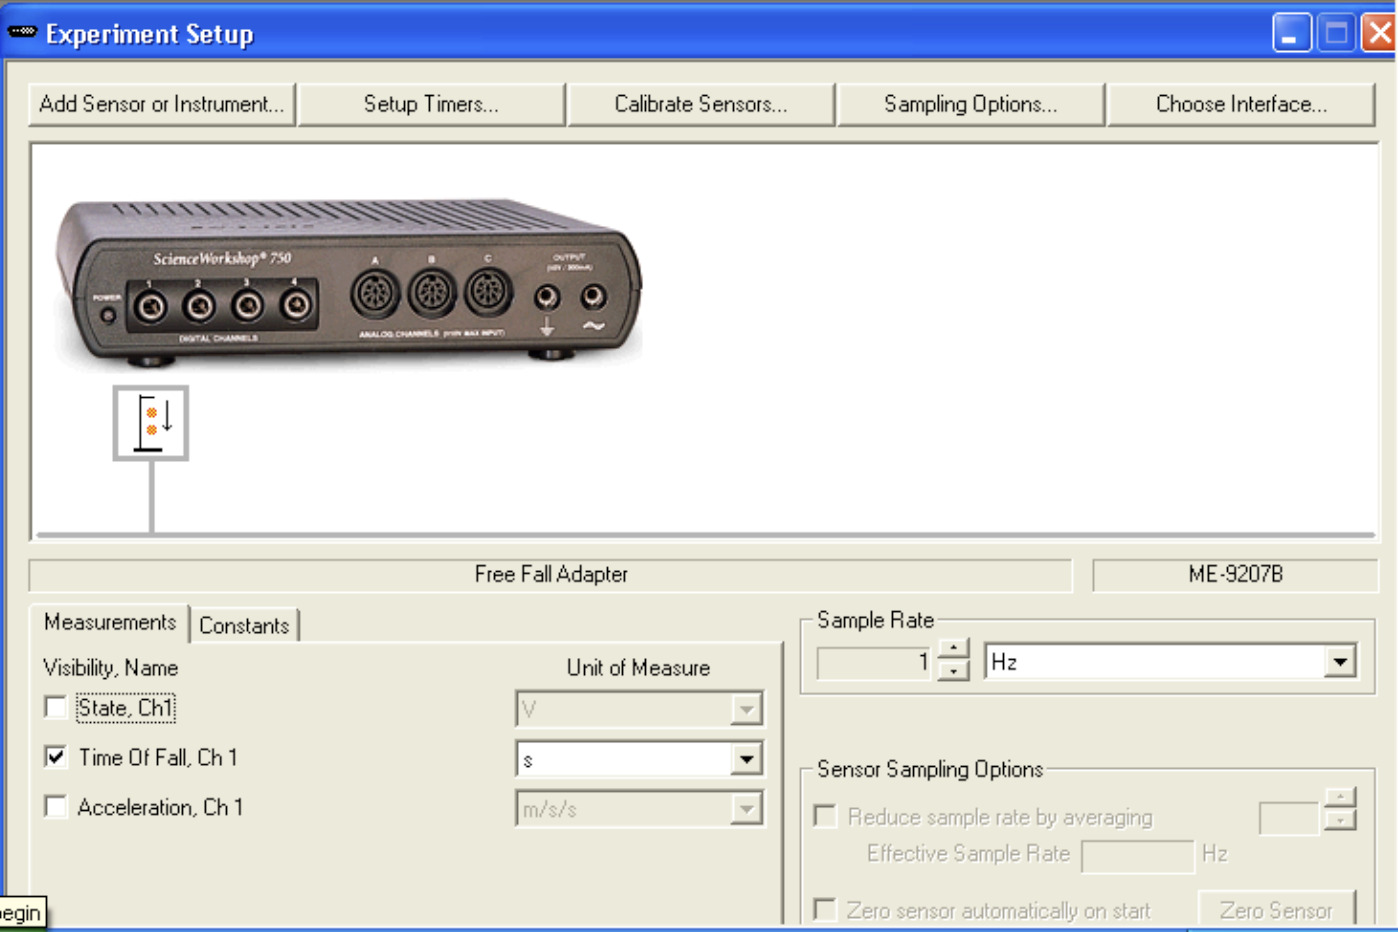
\includegraphics[scale=0.3]{resources/photo4.jpg}}
  \caption{Plug the \emph{Free Fall Adapter} into the channel indicated (here it is in Channel 1).
Click the \emph{Sampling Options} button (located on the top of the \emph{Experiment Setup} window). Make the selections as below:}
\label{3.1}
\end{figure}


\begin{figure}[ht]
  \centerline{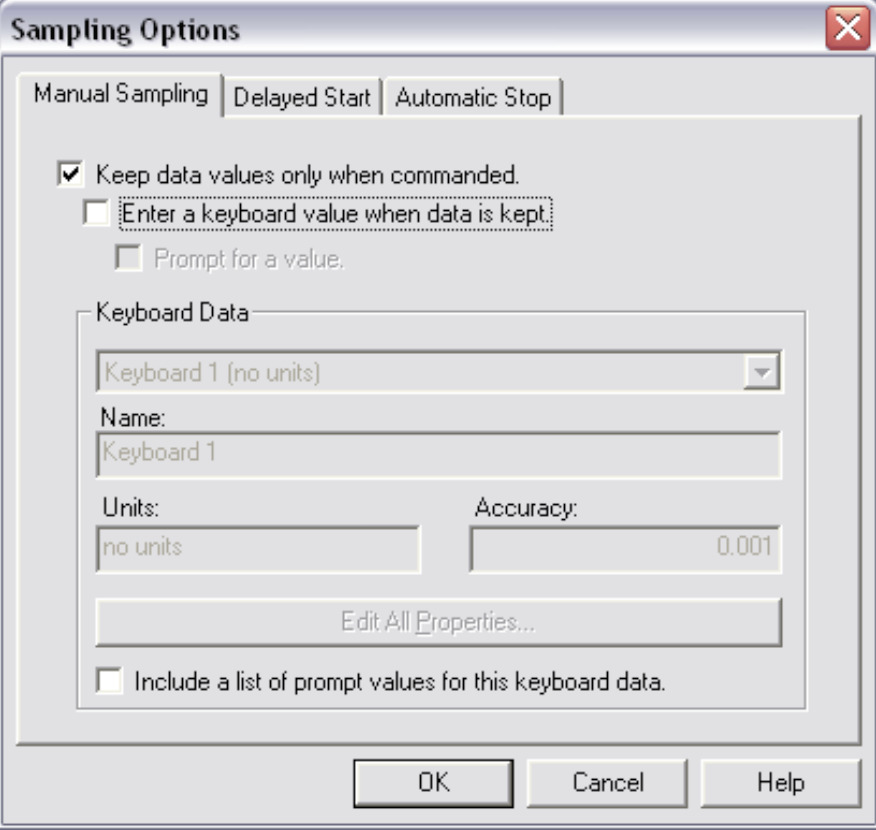
\includegraphics[scale=0.4]{resources/photo5.jpg}}
  \caption{When you click on \emph{“Keep data values only when commanded,”} you will have 
    to uncheck \emph{“Enter a keyboard value when data is kept.”} Click \emph{Ok}. The computer 
    is now ready to collect data.}
  \label{3.2}
\end{figure}

\section{C. Data Collection Setup}

On the left-hand side of the Data Studio program, there are two windows: \emph{Data}
and \emph{Displays}. 

\emph{Data} shows you what you are going to collect. Here, you can see that the only 
data being collected is the \emph{Time of Fall}, in seconds.

\emph{Displays} gives you several choices and formats in which to display your captured 
data. In this lab, we are only going to be concerned with the \emph{Table} display.
We will explore other displays in subsequent labs.

Double-Click \emph{Table} in Displays and select \emph{Time of Fall, Ch 1 (s)}. Click \emph{OK}. 
The following table will appear on your screen:


\begin{figure}[ht]
  \centerline{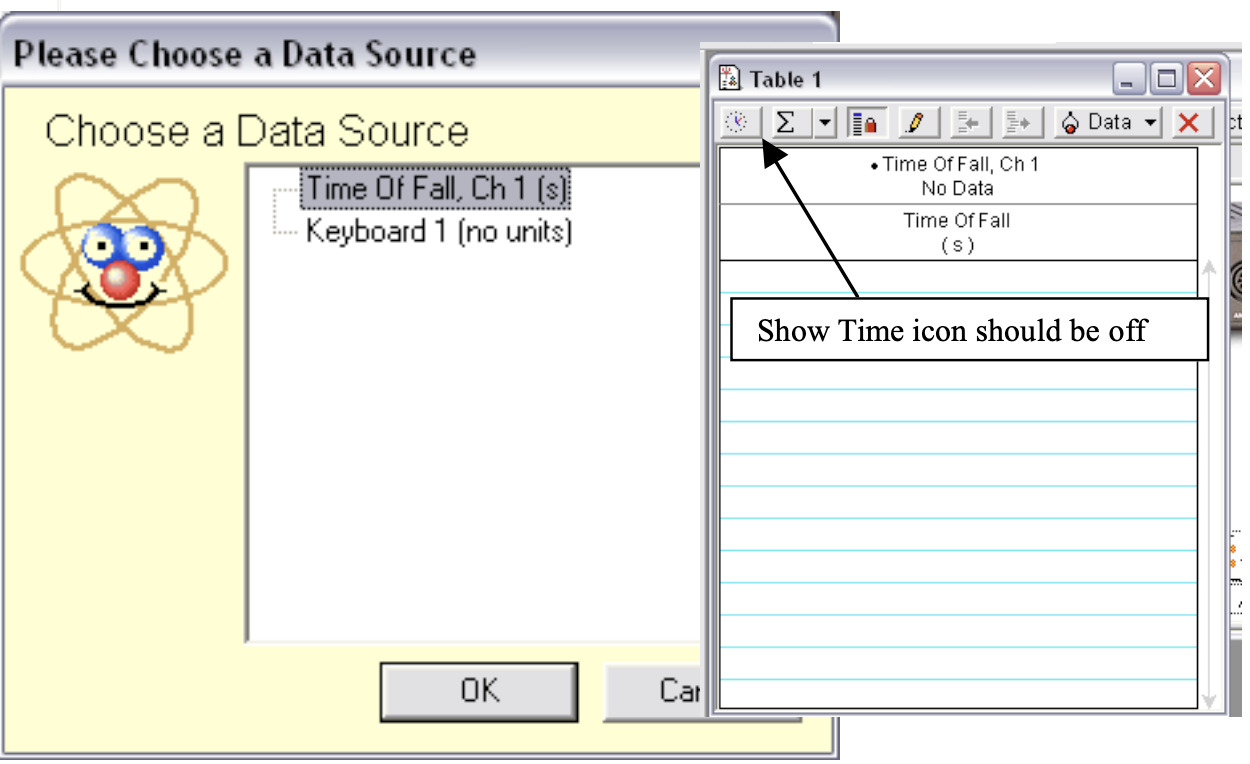
\includegraphics[scale=0.4]{resources/photo6.jpg}}
  \caption{Make sure that the \emph{Show Time} icon, on the top of your table, is \textbf{off}. 
  You are now ready to begin the experiment.}
  \label{3.3}
\end{figure}

\section{D. Data Collection}

  The goal of this experiment is to capture the time it takes the ball to fall a certain distance.
We have set up the computer and apparatus to assist us in capturing the data required.

  You will be dropping each ball over a minimum of 5 distances 
(0.2 m, 0.4 m, 0.6 m,0.8 m, 1.0 m, etc.). Drop the ball 5 times per height 
to get an average time.

  Load the apparatus with the large ball, and set the apparatus at the correct 
height. Click the Start button; this will start the timer. Leave it on 
for the remainder of the experiment. When you drop the ball, the data will 
appear on the table. If it appears to be good data, click the \emph{Keep} button

% \begin{figure}[ht]
%   \centerline{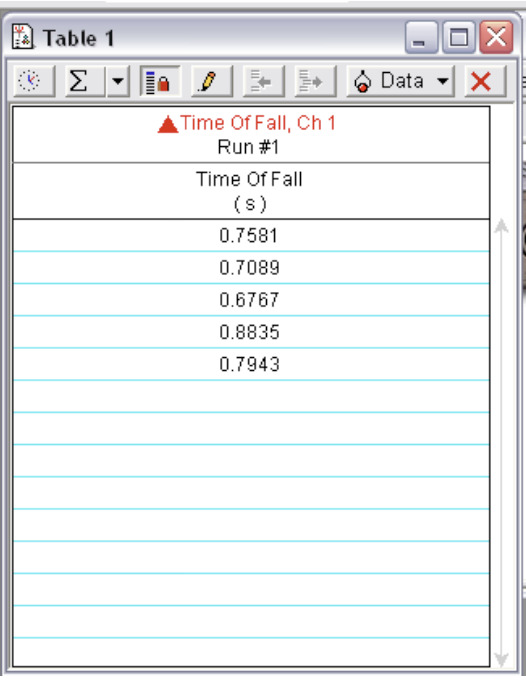
\includegraphics[scale=0.6]{resources/photo7.jpg}}
%   \caption{Repeat 5 times for the given height and press Stop. You can rename 
%   the run to help keep track of where you are in the process (ie. 0.2 m, 1⁄2” 
%   Ball) by clicking on the Run \# Label in the \emph{Data} window.}
%   \label{3.4}
% \end{figure}

% \begin{figure}[ht]
%   \centerline{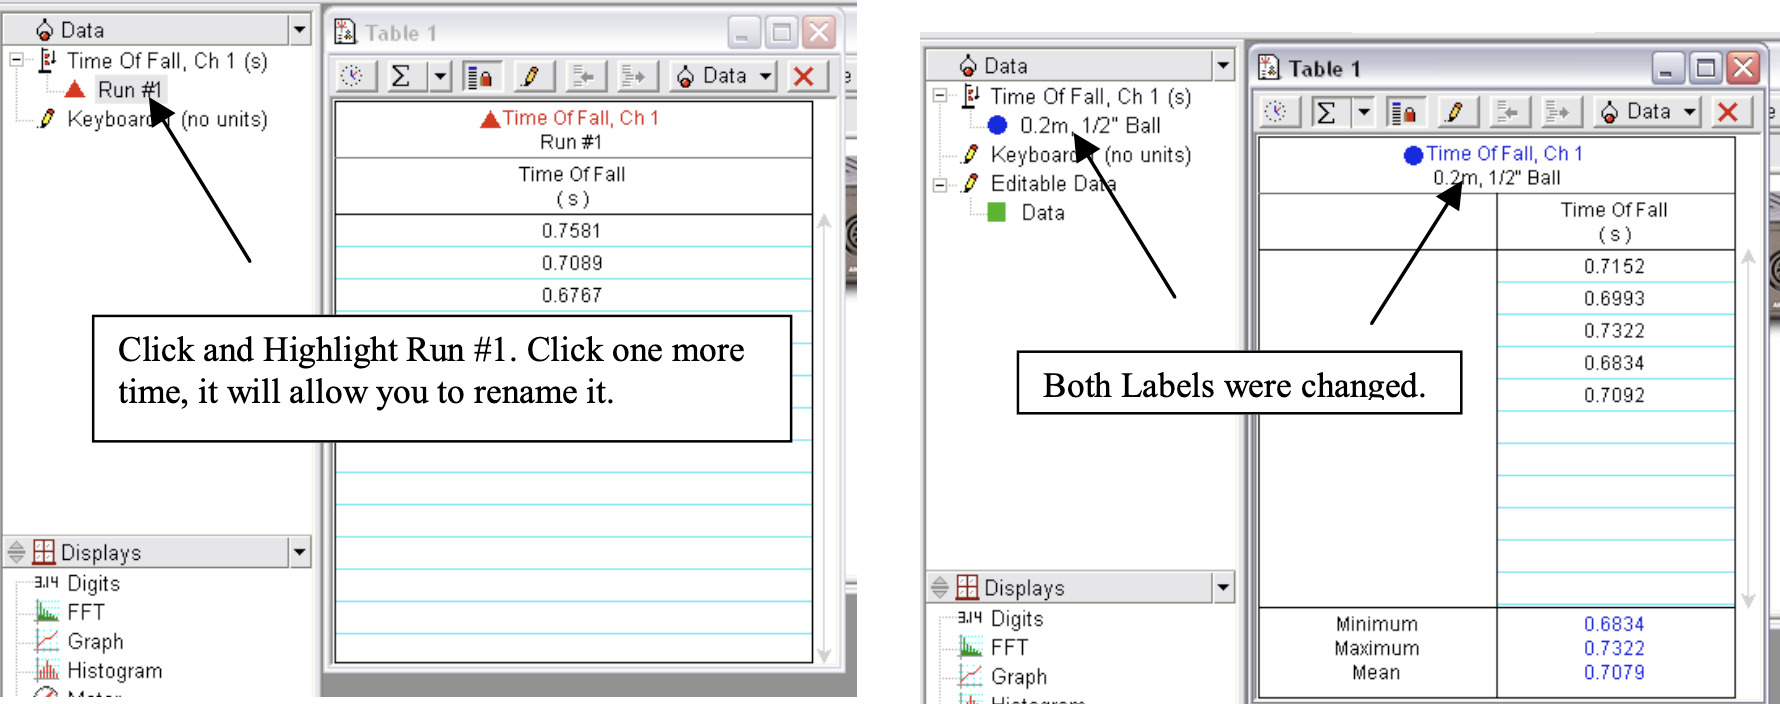
\includegraphics[scale=0.45]{resources/photo8.jpg}}
%   \caption{This is your first set of times. Repeat the experiment at the same height with the smaller ball.
%     Set the apparatus at a new height and repeat. Note: Every time you start and stop the timer, you create new runs.
%     It is possible to delete a run if necessary, Click Experiment \rightarrow}
%     \label{3.5}
%   \end{figure}
  
%   Delete Last
%   Data Run. Caution\: In Data Studio you can only delete the last data run or ALL 
%   data runs, however, once all of the runs have been completed, you will move the 
%   data from each table into Excel for analysis. In \emph{Excel} you can delete any bad data 
%   runs that you were unable to delete in Data Studio.\\
%   You should have at least 5 tables of times per ball, each properly labeled 
%   and ready for transfer into \emph{Excel}. If the data tables are not all open, then 
%   go to the left-hand side of the Data Studio program, where the \emph{Data and 
%   Displays} windows are. Click (and hold) on your data run, then drag it to the 
%   \emph{Table} icon under \emph{Displays} and release the mouse button. A table of that data 
%   run should appear, showing the time of fall.
